\documentclass{article}

% if you need to pass options to natbib, use, e.g.:
%     \PassOptionsToPackage{numbers, compress}{natbib}
% before loading neurips_2018

% ready for submission
% \usepackage{neurips_2018}

% to compile a preprint version, e.g., for submission to arXiv, add add the
% [preprint] option:
    \usepackage[preprint]{neurips_2019}

% to compile a camera-ready version, add the [final] option, e.g.:
 %    \usepackage[final]{neurips_2018}

% to avoid loading the natbib package, add option nonatbib:
%     \usepackage[nonatbib]{neurips_2018}

\usepackage[utf8]{inputenc} % allow utf-8 input
\usepackage[T1]{fontenc}    % use 8-bit T1 fonts
\usepackage{hyperref}       % hyperlinks
\usepackage{url}            % simple URL typesetting
\usepackage{booktabs}       % professional-quality tables
\usepackage{amsfonts}       % blackboard math symbols
\usepackage{nicefrac}       % compact symbols for 1/2, etc.
\usepackage{microtype}      % microtypography
\usepackage{subcaption}
%\usepackage{amsthm}
\usepackage{amssymb}
\usepackage{mathtools}
\DeclarePairedDelimiter\abs{\lvert}{\rvert}
\DeclarePairedDelimiter\norm{\lVert}{\rVert}
\DeclarePairedDelimiter\inner{\langle}{\rangle}
\def\P{\mathcal{P}}
\DeclarePairedDelimiter\floor{\lfloor}{\rfloor}
\DeclarePairedDelimiter\ceil{\lceil}{\rceil}

\DeclareMathOperator*{\argmin}{argmin}

\usepackage{algorithm}
\usepackage{algorithmic}
\makeatletter
\newcommand{\algorithmicfunction}{\textbf{function}}
\newcommand{\algorithmicendfunction}{\algorithmicend\ \algorithmicfunction}
\newenvironment{ALC@func}{\begin{ALC@g}}{\end{ALC@g}}
\newcommand{\FUNCTION}[2][default]{\ALC@it\algorithmicfunction\ #2\ %
\textbf{:}%
\ALC@com{#1}\begin{ALC@func}}
\ifthenelse{\boolean{ALC@noend}}{
    \newcommand{\ENDFUNCTION}{\end{ALC@func}}
  }{
    \newcommand{\ENDFUNCTION}{\end{ALC@func}\ALC@it\algorithmicendfunction}
  }
\makeatother

\title{A practical information theoretic clustering method}

% The \author macro works with any number of authors. There are two commands
% used to separate the names and addresses of multiple authors: \And and \AND.
%
% Using \And between authors leaves it to LaTeX to determine where to break the
% lines. Using \AND forces a line break at that point. So, if LaTeX puts 3 of 4
% authors names on the first line, and the last on the second line, try using
% \AND instead of \And before the third author name.

\author{
  anonymous
}

\begin{document}
% \nipsfinalcopy is no longer used

\maketitle

\begin{abstract}
We propose a graph-based hierarchical clustering method based on a multivariate information metric.
The proposed method can generate non-binary hierarchical tree that reveals the intrinsic structures in the data, with no hyper-parameter to tune. 
The hierarchical tree can be computed efficiently by 
invoking parametric maximum flow algorithm. 
Experiments show that the clustering result outperforms
other hierarchical clustering techniques and is very suitable to find the complex community structure.
\end{abstract}

\section{Introduction}
In traditional agglomerative clustering method, two clusters are agglomerated based on pairwise inter-cluster similarity.  For example, well-known single-linkage clustering method uses nearest distance metric between two clusters and merge the two with minimal distance\cite{RN16}.  However, pairwise comparision is not optimal since it loses information shared between more than two clusters.  To overcome this problem, we define a multivariate similarity measure starting from arbitrary pairwise similarity metrics. Using this multivariate measure in the agglomerative clustering case, we merge several clusters in one step with largest similarity and build our hierachical tree.

The multivariate measure we proposed is equivalent to graph strength \cite{RN12}, it measures the coherrent similarity shared by each component. However, this measure is compute expensive in its definitional form and cannot be used directly to merge clusters. A similar hierachical clustering method called \textbf{minimum average cost} exploits the structural property of the average cost and converts the problem to submodular function minimization\cite{RN7}. In this paper, we show that the same mathematical technique can be used and the special form of submodular function minimization is equivalent to principal sequence of partition\cite{RN3}, which can be solved efficiently by parametric maximal flow algorithm\cite{RN4}. 

The clustering method used in this paper is information theoretic since it is established on the mathematical theory of \textbf{info-clustering}\cite{RN1}. This theory mainly deals with random variable clustering and we generalize and realize it to data clustering scenario, which is the main contribution of this paper. Experiment on synthesized and real-world dataset shows the info-clustering method performs well. 

The paper is organized as follows. In Section \ref{sec:models}, we formulate the info-clustering problem and show its connection with theory. In Section \ref{sec:algorithm}, we propose the algorithm workflow to solve the info-clustering problem. In Section \ref{sec:experiment}, we give the experiement result and comparision of info-clustering with other methods. Finally, we give the conclusion in Section \ref{sec:conclusion}.

Throughout this paper, the graph is denoted by $G(V,E)$, with vertex set $V = \{1, 2, \dots, \abs{V}\}$ and edge set $E=\{(i,j) | w_{ij}>0\}$\footnote{$(\cdot, \cdot)$ is ordered pair. For undirected graph $(i,j) \in E \Rightarrow (j,i) \in E$}. $\P$ is a partition of $V$ and $\{V\}$ is a trival partition. $\Pi$ is the collection of all partitions of $V$. $\Pi' = \Pi \backslash \{V\}$ is the collection of non-trival partitions. $f(\cdot)$ is graph cut function, that is $f(C) = \sum_{i\not\in C, j\in C, (i,j) \in E} w_{ij}$. $f[\cdot]$ is function defined on $\Pi$, that is
\begin{equation}
f[\P] = \sum_{\substack{i\in C, j \not\in C\\ (i,j)\in E, C\in \mathcal{P}}} w_{ij} =
\begin{cases}
\frac{1}{2} \sum_{C\in \P}f(C)   & G \textrm{ is undirected} \\
\sum_{C\in \P}f(C)   & G \textrm{ is directed}
\end{cases}
\end{equation}
An important observation is that if we add direction to an undirected graph, the value of $f[\P]$ is unchanged. Therefore, without specific declaration, $G$ is directed throughout the paper. Given a $\abs{V}$ dimensional vector $x, x(C)=\sum_{i \in C} x_i, C\in V$.
\section{Models}\label{sec:models}

Consider an undirected graph partition problem, in which we want to partition the graph nodes into several groups with largest similarity within each group and smallest similarity between different group. To formulate this problem mathematically, given $G(V, E)$ where the edge weight $w$ is nonnegative and represents pairwise similarity of nodes, we try to minimize the following quantity over different parition of $V$.
\begin{definition}[Multivariate similarity]\label{def:ms}
\begin{align}
I_{\P}(Z_V) & = \frac{ f[\P] }{  \abs{\mathcal{P}} - 1 }\\
I(Z_V) & = \min_{\mathcal{P} \in \Pi'(V)} I_{\mathcal{P}}(Z_V)  \label{eq:ms}
\end{align}
\end{definition}

We call the quantity in equation \eqref{eq:ms} \textbf{multivariate similarity} because it measures the similarity shared by multiple graph nodes. The definition has the same form with that of graph strength if  the whole graph nodes are considered\cite{RN12}. However, we can compute multivariate similarity for any subset of $V$. In such case, 
we use subgraph symbol $V'$ to replace $V$ in equation \eqref{eq:ms}.
\begin{example}\label{eg:three}
For a three node directed graph (See Fig \ref{fig:tn}) $G=(\{1,2,3\},\{(1,2),(1,3),(2,3)\}$ with $w_{12}=w_{23}=1, w_{13}=5\}$, we have $I(Z_{\{1,3\}}) = 5$ and $I(Z_V) = 2$ which is minimal value among $I_{\{1\},\{2\},\{3\}}(Z_V)=3.5, I_{\{1, 2\},\{3\}}(Z_V)=6, I_{\{1,3\},\{2\}}(Z_V)=2, I_{\{1\},\{2,3\}}(Z_V)=6$.(see also \cite{RN9} Fig. 1)
\end{example}

Based on the definition \eqref{def:ms}, we have both a top-down and bottom-up version of hierachical clustering.

\begin{proposition}\label{prop:ta}
The following two procedures generate the same hierachical tree.
\begin{enumerate}
\item For a graph $G$, suppose $I_{\P}(Z_V)=I(Z_V)$, each subset of $\P$ is child of hierachical tree root $V$. For each tree leaf node set $C$, use partition $\P_C$($I(Z_C)=I_{\P_C}(Z_C)$) to split it until the leaf node has exactly one element.
\item For a graph $G$, suppose $I(Z_C) = \max_{B\subseteq V} I(Z_B)$ and $C$ is maximal, merge singleton element of $C$ together and $G$ is contracted. At each step select the set with maximal multivariate similarity to contract the graph until the graph contracted to one vertex.
\end{enumerate}
\end{proposition}
%proof in attachment.
The two procedures are illustrated by figure \ref{fig:ta}. For the top-down approach, there may be multiple partition $\P$ that reaches the minimum in \eqref{eq:ms}, we can show that there is a unique finest partition and this one is used; for the bottom-up approach, there may be multiple intersecting subsets with equal maximal multivariate similarity, we can show that the union of these subsets also reach the maximal and maximal $C$ is unique.
%proof in attachment, before the proof of the above proposition. (2 statements)
\begin{figure}
\centering
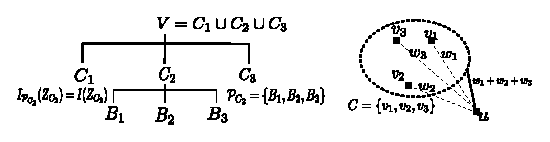
\includegraphics[width=0.8\textwidth]{pic/two_approach.eps}
\caption{hierachical tree generation based on multivariate similarity. Left figure shows the top-down approach with each subset splitted. Right figure shows the bottom-up approach with the graph contracted.}\label{fig:ta}
\end{figure}

By the construction of the clustering tree, we can associate each tree node with a threshold value, which is multivariate similarity computed at that step.
\begin{example}
\begin{figure}
\centering
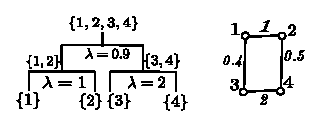
\includegraphics[width=0.8\textwidth]{pic/threshold.eps}
\caption{a clustering tree (left figure) for the weighted graph (right figure) by info-clustering method. Threshold values are $0.9, 1, 2$.}\label{fig:threshold}
\end{figure}
Consider an undirected graph $G(V, E)$ with $V=\{1,2,3,4\}$ and $E=\{(1,2),(1,3),(3,4),(2,4)\}$ with edge weight $w_{12}=1,w_{13}=0.4,w_{24}=0.5,w_{34}=2$ (See Fig. \ref{fig:threshold}). The threshold values are the multivariate similarity $I(Z_{3,4})=2, I(Z_{1,2})=1$ and $I(Z_V)=0.9$ respectively. We can write the complete clustering solution as:
\begin{equation*}
\P = 
\begin{cases}
\{\{1,2,3,4\}\} & \lambda < 0.9 \\
\{\{1,2\},\{3,4\}\} & 0.9 \leq \lambda < 1 \\
\{\{1\},\{2\},\{3,4\}\} & 1 \leq \lambda < 2\\
\{\{1\},\{2\},\{3\},\{4\}\} & \lambda \geq 2
\end{cases}
\end{equation*}
Although the clustering tree does not distinguish $\{\{1\},\{2\},\{3,4\}\}$ with $\{\{1,2\},\{3\}, \{4\}\}$ ,Notice that partition $\{\{1,2\},\{3\}, \{4\}\}$ does not exist by the threshold method.
\end{example}
Using $I(Z_V)$ to cluster data directly is computing expensive, the same clustering result can be achieved by solving the following optimalization problem for all $\lambda$ (Corollary 2 in \cite{RN1}).
\begin{theorem}\label{thm:psp}
\begin{equation}\label{eq:hL}
h(\lambda) = \min_{\P \in \Pi'(V)}\{ f[\P] - \abs{\P} \lambda \}
\end{equation}
The optimal partitions for $h(\lambda)$ are finite and they can be arranged in a decrasing sequence $\P_1, \dots, \P_k$ such that $\P_1 \succeq \P_2 \dots \succeq \P_k$, This sequence is called \textbf{principal sequence of partitions} of $h(\lambda)$(proved in \cite{RN3}).
\end{theorem}
%proof in attachment

For given $\P$, the function about $\lambda$ is linear, therefore $h(\lambda)$ is piecewise linear and each turning point of $h(\lambda)$ corresponds to $\P_i, \P_{i+1}$ respectively. We can use the parametric maximal flow algorithm to compute $\P_i$ efficiently, which is shown in the next section.

The method is information theoretic since it is an extension of mutual information in information theory. When the graph node is random variable and the edge weight is mutual information metric, then equation \eqref{eq:ms} becomes one form of multivariate mutual information proposed in \cite{RN1}. When $I(Z_V)=0$, the random variables $Z_i$ are pairwise independent. 

Info-clustering assume the weight is additive and tends to produce trival hierachical structure when the value of weights are near equal. This is shown by the following theorem:
\begin{theorem}\label{thm:trival}
The paritition to minimize equation \eqref{eq:ms} is $\{\{1\},\{2\},\dots,\{\abs{V}\}\}$ if and only if equation \eqref{eq:GF} holds.
\begin{equation}\label{eq:GF}
\frac{f[\P]}{\abs{\P}-1} \geq \frac{\sum w_{ij, (i,j) \in E}}{\abs{V}-1} \textrm{ for any } \P \in \Pi'
\end{equation}
\end{theorem}
\begin{proof}
Since $h(\lambda)$ is piecewise linear, the first line segment of $h(\lambda)$ is $ - \lambda $ and the last line segment is $ \sum w_{ij, (i,j) \in E} - \abs{V} \lambda$. Their intersection point is $(\lambda_{+}, -\lambda_{+})$ where $\lambda_{+} = \frac{\sum w_{ij, (i,j) \in E}}{\abs{V}-1}$. Since $\frac{f[\P]}{\abs{\P}-1} \geq \lambda_{+} \iff f[\P] - \abs{\P}\lambda_{+} \geq - \lambda_{+}$ Equation \eqref{eq:GF} says the minimzer of $h(\lambda)$ at $\lambda = \lambda_{+}$ is either $\{V\}$ or $\{\{1\},\{2\},\dots,\{\abs{V}\}\}$ and $h(\lambda)$ has only two line segments. From geometric point of view, the solution to equation \eqref{eq:ms} is the first turning point of $h(\lambda)$ and it is equal to that of last turning point if and only if \eqref{eq:GF} holds.
\end{proof}
By theorem \ref{thm:trival}, we can show that all weights are of equal value, then by applying info-clustering we can only get each data point as a cluster. Generally, we have the following proposition.
\begin{proposition}\label{prop:triangle}
Let $w_{ij}=0$ if $(i,j)\not\in E$. If $w_{ij} + w_{jk} \geq w_{ki}$ for any different triple $i, j, k \in V$, then the info-clustering solution is trivial\footnotemark.
\end{proposition}
\footnotetext{By trivial solution we mean only $\{V\}$ is a cluster, or the hierarchical tree contains only root and leaves.}
It inspires us in order to seperate different clusters, we need small magnitude of inter cluster weights and large and similar weight value of intra cluster.

\section{Algorithm}\label{sec:algorithm}

In this section, we review the basic theory to solve equation \eqref{eq:hL} and propose an improved algorithm flow based on the work of \cite{RN4}.

Since $h(\lambda)$ is piecewise linear, we can use divide and conquer to search the turning points and evaluate $h(\lambda)$ only at these turning points. This is the method proposed at \cite{RN7} and has complexity $N^2 \mathtt{MaxFlow}(N)$ if the hierachical tree structure is needed. If we are only interested in finding a suitable partition  with at least $k$ part, then the algorithm complexity can be reduced to $\log(N) N \mathtt{MaxFlow}(N)$. This is the approach evaluated at subsection \ref{sec:fc}.

We call this aprroach Dilworth truncation. It solves \eqref{eq:hL} for fixed $\lambda$ by solving the following equation sequentially for $t=1,\dots,\abs{V}$.
\begin{align}\label{eq:pmq}
\tilde{h}(\lambda) & = \min_{t \in T \subseteq V} \tilde{h}_{\lambda}(T) \\
\tilde{h}_{\lambda}(T) &= f(T) - \lambda - y^{\lambda}(T)
\end{align}
where
$y^{\lambda}_i = \min\{a_i - \lambda, b_i\}$  and $b_i \leq +\infty$. 

\begin{figure}
	\centering
	\begin{subfigure}{0.45\textwidth}
		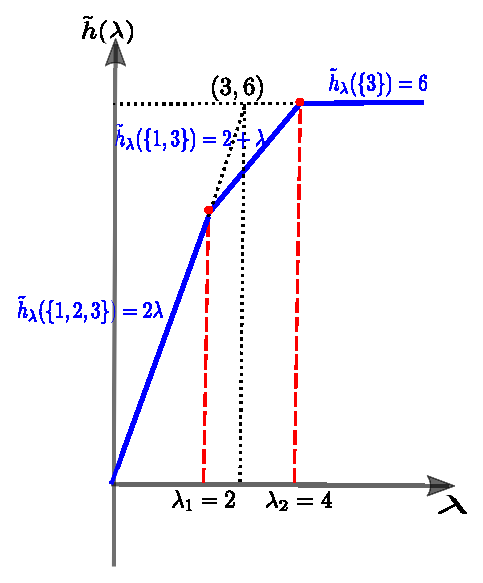
\includegraphics[width=\textwidth]{pic/example_pst_single.eps}
		\caption{An illustration to Algorithm \ref{alg:pmfT}}\label{fig:linseg}
	\end{subfigure}
	\begin{subfigure}{0.45\textwidth}
		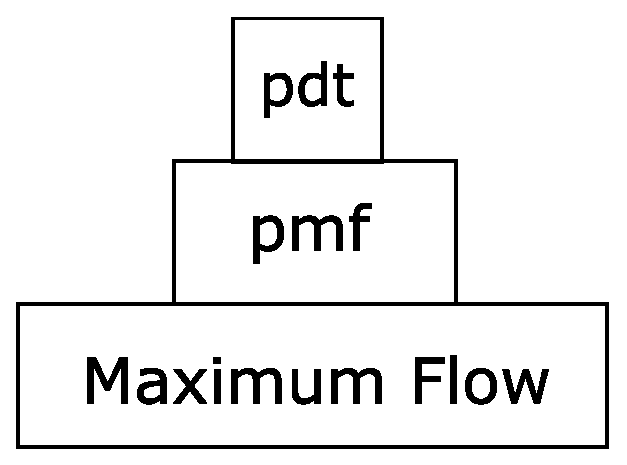
\includegraphics[width=\textwidth]{pic/pdt.eps}
		\caption{Algorithmic pyramid to compute principal sequence of partitions. The top level is parametric Dilworth truncation; the middle level is parametric maximal flow and the bottom level is maximal flow}\label{fig:pyramid}
	\end{subfigure}
\end{figure}

It is pointed out in \cite{RN4} that \eqref{eq:pmq} can be solved with $\lambda$ as a parameter, not a value. We call this method parametric Dilworth truncation(pdt in short, in Fig \ref{fig:pyramid}). It can solve \eqref{eq:hL} directly by treating $\lambda$ as a parameter. However, how to solve \eqref{eq:pmq} for fixed $j$ is not a trival task and the approach given in \cite{RN4} is too complex to analyze. We will give an clear and efficient approach to solve \eqref{eq:pmq} for $\lambda\geq 0$. 

First we have the following property to the solution set of $\tilde{h}(\lambda) $.
\begin{proposition}\label{prop:struc}
If $f$ is a submodular function which satisfies $f(A\cup B) + f(A\cap B) \leq f(A) + f(B)$ and 
let $A^{\lambda}$ be the solution to $\tilde{h}(\lambda)$, then 
\begin{equation}\label{eq:Alambda}
\mathcal{A}^{\lambda}=\begin{cases}
T_0 & \lambda < \lambda_1 \\
T_i & \lambda_i \leq \lambda < \lambda_{i+1}, \textrm{ for } i=1, 2, \dots, k-1 \\
T_k & \lambda \geq \lambda_{k}
\end{cases}
\end{equation}
where $T_k \subsetneq  \dots \subsetneq T_1 \subsetneq T_0$
\end{proposition}

In proposition \ref{prop:struc}, if $\lambda$ is sufficiently large, then all $y_i^{\lambda}$ will have the form $a_i -  \lambda$ and the minimum solution is $\{t\}$. That is, $T_k = \{t\}$; On the other hand, since we are only concerned about $\lambda \geq 0$. We can compute \eqref{eq:pmq} for $\lambda = -\epsilon (\epsilon > 0)$. Then we have $T_0$ and $T_k$ in \eqref{eq:Alambda}.

Another important observation of function $\tilde{h}(\lambda)$ is that it is piecewise linear and concave. $T_0$ corresponds a piecewise linear part and $T_k$ corresponds another one.  To compute the nested family between $T_0$ and $T_k$, we use divide and conquer techniques. The algorithm is presented in Algorithm \ref{alg:pmfT}.
\begin{algorithm}
	\caption{Parametric Computing of $T^{\lambda} = \argmin_{t\in V} g_{\lambda}(T)$}\label{alg:pmfT}
	\begin{algorithmic}[1]
		\REQUIRE set $V$, $t \in V$, function $g_{\lambda}$ whose domain is $V$.
		\ENSURE An ordered array \textbf{L} which contains $\lambda_1, \dots \lambda_k$ and a reversely ordered array $T^{\lambda}$ which contains $T_0,\dots, T_k$. (defined in equation \eqref{eq:Alambda})
		\STATE \textbf{L}, $A^{\lambda} \leftarrow$ empty arrays of size $\abs{V}$
		\STATE $Q \leftarrow \argmin_{A\in V} g_{-\epsilon}(A), P \leftarrow \{ t \}$ \label{alg:uini}
		\STATE add $Q$ and $P$ to $T^{\lambda}$
		\STATE \texttt{Split}$(Q,P)$
		\FUNCTION{\texttt{Split}$(Q,P)$}
		\STATE Let $\tilde{\lambda}_2$ be the solution to $g_{\lambda}(Q) =  g_{\lambda}(P)$
		\STATE $h' = g_{\tilde{\lambda}_2}(Q)$
		\STATE $P' =\argmin_{A\in V} g_{\tilde{\lambda}_2}(A)$  \label{alg:Pap}
		\IF{$ g_{\tilde{\lambda}_2}(P') = h'$}
		\STATE add  $\tilde{\lambda}_2$ to $\mathbf{L}$
		\ELSE
		\STATE add $P'$ to $T^{\lambda}$ \label{alg:addP}
		\STATE \texttt{Split}$(Q,P')$
		\STATE \texttt{Split}$(P',P)$
		\ENDIF
		\ENDFUNCTION
	\end{algorithmic}
\end{algorithm}

\begin{example}
We use the graph defined in Example \ref{eg:three} and define $f$ as the graph cut function, $t=3$ and $y^{\lambda}_i = -\lambda, i=1,2,3$. 
We can get $T_0 = \{1,2,3\} $ and $T_k = \{3\}$. And their corresponding lines are $\tilde{h}_{\lambda}(T_0) =2\lambda$ and $\tilde{h}_{\lambda}(T_k)=6$. As Figure \ref{fig:linseg} shows, they intersect at $(3, 6)$, the set $T_1=\{1,3\}$; and we can compute $\tilde{h}(3)=5<6$. That is, there are turning points of $\tilde{h}$ at interval $(0, 3)$ and $(3, +\infty)$ respectively. For $(0,3)$, we compute the intersection of $\tilde{h}_{\lambda}(T_0)$ and $\tilde{h}_{\lambda}(T_1)=2+\lambda$ and get the intersection coordinate $(2,4)$; Also $\tilde{h}(1)=4$, therefore, the computation for $(0,3)$ is finished. The same goes for $(3, +\infty)$. And finally, we can get $L=[2,4, +\infty]$ and $A^{\lambda} = [\{1,2,3\}, \{1,3\},\{3\}]$	
\end{example}

Algorithm \ref{alg:pmfT} is only theoretically computable. To make it possible to implementation, we need to figure out how to solve $\tilde{\lambda}_2$ and how to compute $\tilde{h}(\lambda)$ for given $\lambda$ efficiently.

To simplify our notation, in this section we will let $w_{ij} = 0$ if $(i,j) \not\in E$. To compute $\tilde{h}(\lambda)$, we combine Algorithm \ref{alg:pmfT} and paramatric maximal flow Algorithm (shorted as pmf in Fig \ref{fig:pyramid}). The combination begins at creating a new weighted directed graph $\widetilde{G}(\widetilde{V}, \widetilde{E})$ from directed graph $G(V,E)$:
\begin{enumerate}
	\item Add a new node $s$ and initialize $c^{\lambda}(s,v)=\max\{0, -y^{\lambda}_v\}$ for $v \in V\backslash \{j\}$
	\item Modify the in arc capacity of node $j$ as $c^{\lambda}(v,t) = w_{vt} + \max\{0, y^{\lambda}_v\}$
	\end{enumerate}
In detailed form, the edge weight is defined by:
\begin{equation}
c^{\lambda}(i, j) = 
\begin{cases}
	\max\{0, -\min\{a_i-\lambda, b_i\}\} &  i = s, j \neq t \\
	w_{it} + \max\{0, \min\{a_i - \lambda, b_i\}\} & i\neq s, j = t\\
	0 & i = s, j = t\\
	w_{ij} & i \neq s, j \neq t
\end{cases}
\end{equation}
\begin{figure}
	\centering
	\begin{subfigure}{0.4\textwidth}
		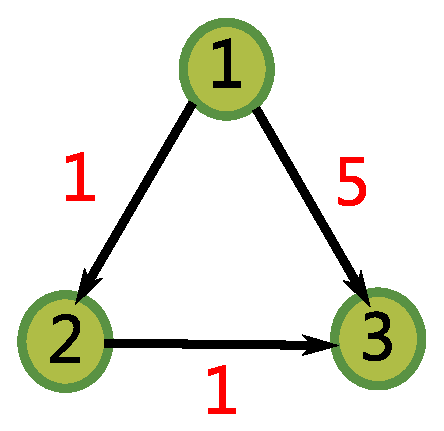
\includegraphics[width=\textwidth]{pic/example_directed.eps}
		\caption{An example graph $G$ with three nodes}\label{fig:tn}
	\end{subfigure}~
	\begin{subfigure}{0.4\textwidth}
		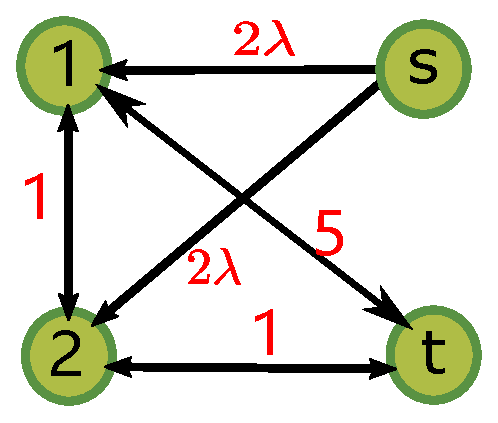
\includegraphics[width=\textwidth]{pic/example_st.eps}
		\caption{$\widetilde{G}$ derived from left graph with $t=3$}\label{fig:tn_converted}
	\end{subfigure}
	\caption{}
\end{figure}
For $\widetilde{G}(\widetilde{V}, \widetilde{E})$, there are two special nodes $s$ and $j$, The s-t cut for $\widetilde{G}$
is defined as $c^{\lambda}(T) = \sum_{i \not\in T, j \in T} c^{\lambda}(i,j)$ where $s \not\in T, t \in T$. By such construction we can guarantee $c^{\lambda}(i,j)\geq 0$ and has the following property.
\begin{proposition}\label{prop:constDiff}
	\begin{align}
		\tilde{h}_{\lambda}(T) &= c^{\lambda}(T) - \lambda - \sum_{v \in V} \max\{0, y^{\lambda}_v\}\\
	A^{\lambda}	&= \argmin_{s\in U\backslash T, t\in T}c^{\lambda}(T) \label{eq:pmqe}
	\end{align}
\end{proposition}
\begin{proof}
	
	\begin{align*}
	c^{\lambda}(T) &= f(T) + \sum_{i \not\in T} (c^{\lambda}(i, t) - w_{it})+ \sum_{j \in T} c^{\lambda}(s,j) \\
	\Rightarrow \tilde{h}_{\lambda}(T) - c^{\lambda}(T) &= -\lambda - \sum_{j \in T} y^{\lambda}_j - \sum_{i \not\in T} \max\{0, y^{\lambda}_i\} - \sum_{j \in T} \max\{0,-y^{\lambda}_j\}\\
	&= -\lambda - \sum_{v \in V} \max\{0, y^{\lambda}_v\}
	\end{align*}
\end{proof}

By proposition \ref{prop:constDiff}, for a given $\lambda, \tilde{h}_{\lambda}$ and $c^{\lambda}$ differs a constant value for any $T\subseteq V$. Therefore, we can use $c^{\lambda}$ in Algorithm \ref{alg:pmfT} such that $\argmin c^{\lambda}$ can be computed by maximal flow algorithm. 

Within function \texttt{Split} in Algorithm \ref{alg:pmfT}, An important notice is that we do not compute $P'$ in line \ref{alg:Pap} refreshly but starting from a given flow map which is max flow when computing $Q$. By doing so, the time complexity to minimize $c^{\lambda}$ is reduced to $O(N\abs{E})$ and the bottleneck is the uninitialized minimization at line \ref{alg:uini}, which is $O(N^2\sqrt{E})$ when highest-label selection rule is used.

The result of top level routine is a nested family of partition and its corresponding turning point. In example \ref{eg:three}, we have $[\{1,2,3\},\{\{1,3\},\{2\}\},\{\{1\},\{2\},\{3\}\}],[2,5,+\infty) $ as a return. At the middle level, one of graph node is treated as sink node and parametric maximal flow(pmf) routinue is called.

The pmf routinue is called $\abs{V}$ times. At the bottom level, the edge cost is fixed for given $\lambda$ and maximal flow routinue is called. By the analysis in \cite{RN17}, the time complexity for pmf is the same with that of maximal flow.

For the pmf algorithm applied to our problem, we are required to solve 
We can make the parameter dependent part on the edge cost and turn the undirected graph to the directed graph by splitting each edge into two directed arc with same capacity value. We also introduce a source
node $s$ while $j$ is treated as target node.  then change
$c^{\lambda}(s,v)=\max\{0, -y^{\lambda}_v\}, c^{\lambda}(v,j) += \max\{0, y^{\lambda}_v\}$ for $ v=1 $ to $\abs{V}$ and $v \neq  j$. Then we claim that



\section{Experiment}\label{sec:experiment}
In this section, we demonstrate info-clustering algorithm on two kinds of datasets. The first is about feature clustering, in which we need to cluster multi-dimentional vectors. For this kind of task, we need to construct the clustering graph first by using proper similarity measure. The other dataset is in community detection, coming from \cite{RN22}, in which a two-level hierachical structure is defined. By comparision with other clustering method, we will show that info-clustering algorithm gives reasonable good result and can recover the two-level hierachical structure under certain conditions. 

\subsection{Feature Clustering}\label{sec:fc}
For feature clustering task, we prepare three groups of data:
\begin{enumerate}
\item Four Gaussian blobs with unit variance and centers at $(3,3), (3,-3), (-3,3), (-3,-3)$.  We generate 25 points for each blob.
\item Three concentric circles with radius $0.1,0.2,0.3$ and number of data points as $60, 100, 140$. The angles of these points are uniform distributed and they also oscillate around the radius direction.
\item Iris flower dataset with 50 samples, 3 classes, 4 dimensions of feature.
\end{enumerate}
We use adjusted rand index as the clustering metric to score different clustering method, the best performance for each algorithm is shown in Table \ref{tb:e1}.  It can be seen from the table that info-clustering algorhthm is competitive with other clustering algorithms.
\begin{table}
\centering
\InputIfFileExists{build/compare_3.tex}{}{}
\caption{ accuracy for different clustering algorithms }\label{tb:e1}
\end{table}
\subsection{Community Detection}
For community detection task, we use a two-level artifical dataset proposed in \cite{RN22}. 
The community structure is shown in Figure \ref{fig:c1}. In macro-level, it has 4 communities and each macro community contains 4 micro communities. We use $z_{\mathrm{in}_1}$ to represent the internal average degree of nodes within micro community; $z_{\mathrm{in}_2}$ as node degree between different micro communities but within one macro community; $z_{\mathrm{out}}$ as node degree between different macro communities. By varying one and fixing the other two in $\{z_{\mathrm{in}} , z_{\mathrm{in}_2}, z_{\mathrm{out}} \}$ we get different set of experiment and in each given community parameter, we compare the detection accuracy between different methods. The result is shown in Table.

It is noticed that for such problems with unweighted graph, it is more practical to deduce a weighted graph with the weight value defined as 
\begin{equation}
    w_{ij} = 1 + \abs{\{k | (i,k),(j,k) \in E \}} \textrm{ for } (i,j) \in E
\end{equation}
This is the number of triangles which contain the edge. Such definition is justified by the following proposition.
\begin{proposition}
Suppose $S_1, S_2 $ are complete graph with $n$ nodes and equal weight $w=n$. There are $m$ edges between the two graphs and all inter-connection edge is with equal weight 1. Then we have
\begin{equation}
I(Z_V) = \begin{cases}
m & m <\frac{n^2}{2}, S_1,S_2 \textrm{ are non-trival cluster} \\
\frac{m+n^2(n-1)}{2n-1} & m\geq \frac{n^2}{2}, \textrm{ only trival cluster exists} 
\end{cases}
\end{equation}
\end{proposition}
This proposition inspires us to increase the weight linearly with the number of nodes for densely connected part of the whole community. It increases the performance of info-clustering algorithm.

\begin{figure}
\centering
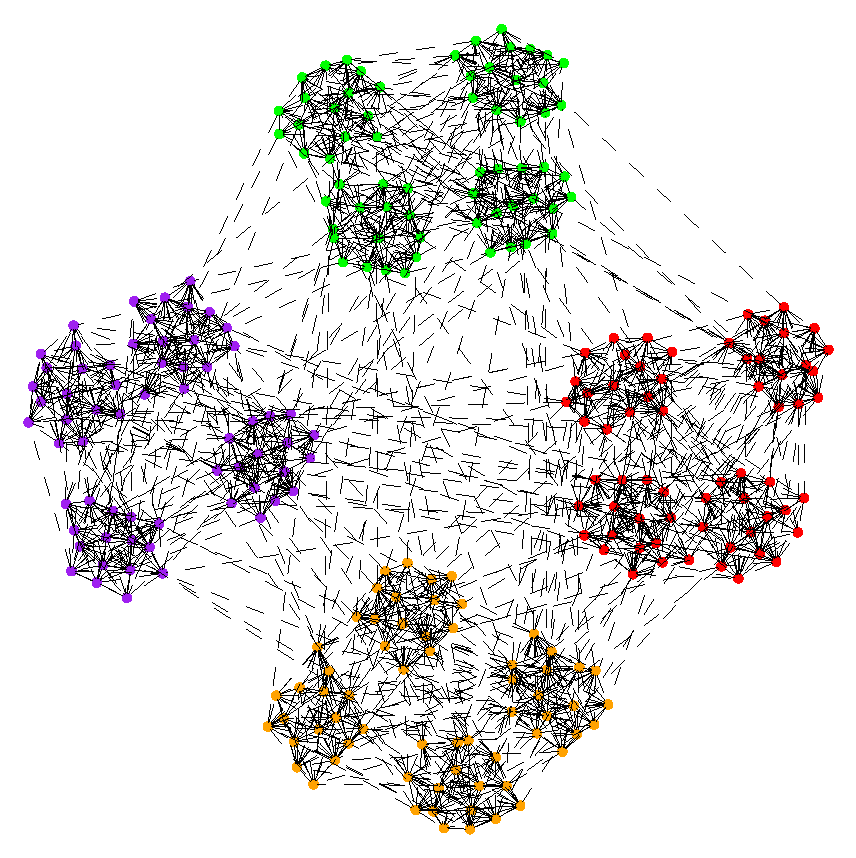
\includegraphics[width=6cm]{pic/two_level.eps}
\caption{a community with 256 nodes, 16 components in micro-level, each 4 components compose a macro-level larger part of this community. $z_{\mathrm{in}_1} = 14, z_{\mathrm{in}_2} = 3, z_{\mathrm{out}}=1$}\label{fig:c1}
\end{figure}

\begin{figure}
\centering
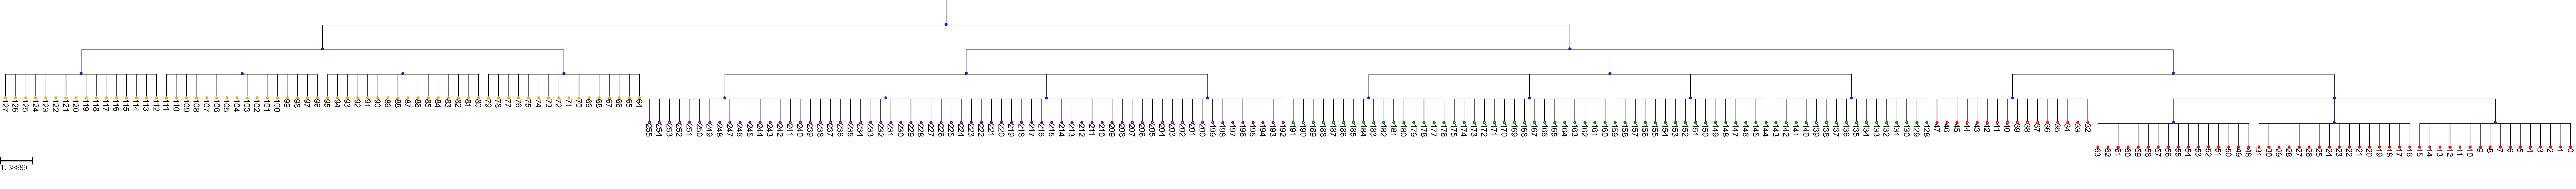
\includegraphics[width=10cm]{pic/tree.pdf}
\caption{a community with $z_{\mathrm{in}_1} = 14, z_{\mathrm{in}_2} = 2.3$ and $z_{\mathrm{out}}=0.1$. The tree depth is only 4.}\label{fig:c2}
\end{figure}

\section{Conclusion}\label{sec:conclusion}


\subsubsection*{Acknowledgments}



\bibliographystyle{plain}
\bibliography{exportlist}


\end{document}
